
\chapter{ACC sectors}
\label{chap:acc:sectors}

\section{Sector division}

Sector division of vFIR Warszawa is shown in \cref{tab:acc:sectors} and \cref{fig:acc:sectors}.

\begin{table}[htbp]
  \centering
  \begin{tabular}{|c l|c|}
    \hline
    \multicolumn{2}{|c|}{\cellcolor{vred}\color{white}\textbf{Sector}}&\cellcolor{vred}\color{white}\textbf{Frequency} [MHz]\\\hline
    \color{Orange}T ALLFIR & \tiny [EPWW\_CTR] & 125.450\\\hline
    \color{OliveGreen}UPPER & \tiny [EPWW\_U\_CTR] & 130.625\\\hline
    \color{ProcessBlue}B & \tiny [EPWW\_B\_CTR] & 127.025\\\hline
    \color{Orange}C & \tiny [EPWW\_C\_CTR] & 133.475\\\hline
    \color{Orange}D & \tiny [EPWW\_D\_CTR] & 134.225\\\hline
    \color{MidnightBlue}E & \tiny [EPWW\_E\_CTR] & 120.950\\\hline
    \color{ProcessBlue}F & \tiny [EPWW\_F\_CTR] & 129.075\\\hline
    \color{ProcessBlue}G & \tiny [EPWW\_G\_CTR] & 124.925\\\hline
    \color{vred}J & \tiny [EPWW\_J\_CTR] & 124.625\\\hline
    \color{MidnightBlue}N & \tiny [EPWW\_N\_CTR] & 132.700\\\hline
    \color{vred}R & \tiny [EPWW\_R\_CTR] & 123.625\\\hline
  \end{tabular}
  \caption{ACC sectors of vFIR Warszawa}
  \label{tab:acc:sectors}
\end{table}

Sector are connected into blocks:

\begin{tabular}{lll}
  \textbf{Block N}&Sectors \textbf{N} and \textbf{E}.& Master sector: \textbf{N}.\\
  \textbf{Block NW}&Sectors \textbf{B}, \textbf{F} and \textbf{G}.& Master sector: \textbf{G}.\\
  \textbf{Block S}&Sectors \textbf{J} and \textbf{R}.&Master sector: \textbf{J}.\\
  \textbf{Block W} & Sectors \textbf{C}, \textbf{D} and \textbf{T}.&Master sector: \textbf{T (ALLFIR)}.\\
\end{tabular}

Blocks are connected into the following groups:

\begin{tabular}{lll}
  \textbf{Group North}&Blocks \textbf{N} and \textbf{NW}.& Master sector: \textbf{N}.\\
  \textbf{Group West}&Block \textbf{W}.&Master sector: \textbf{T (ALLFIR)}.\\
  \textbf{Group South}&Block \textbf{S}.&Master sector: \textbf{J}.\\
\end{tabular}

\begin{figure}[htbp]
  \centering
  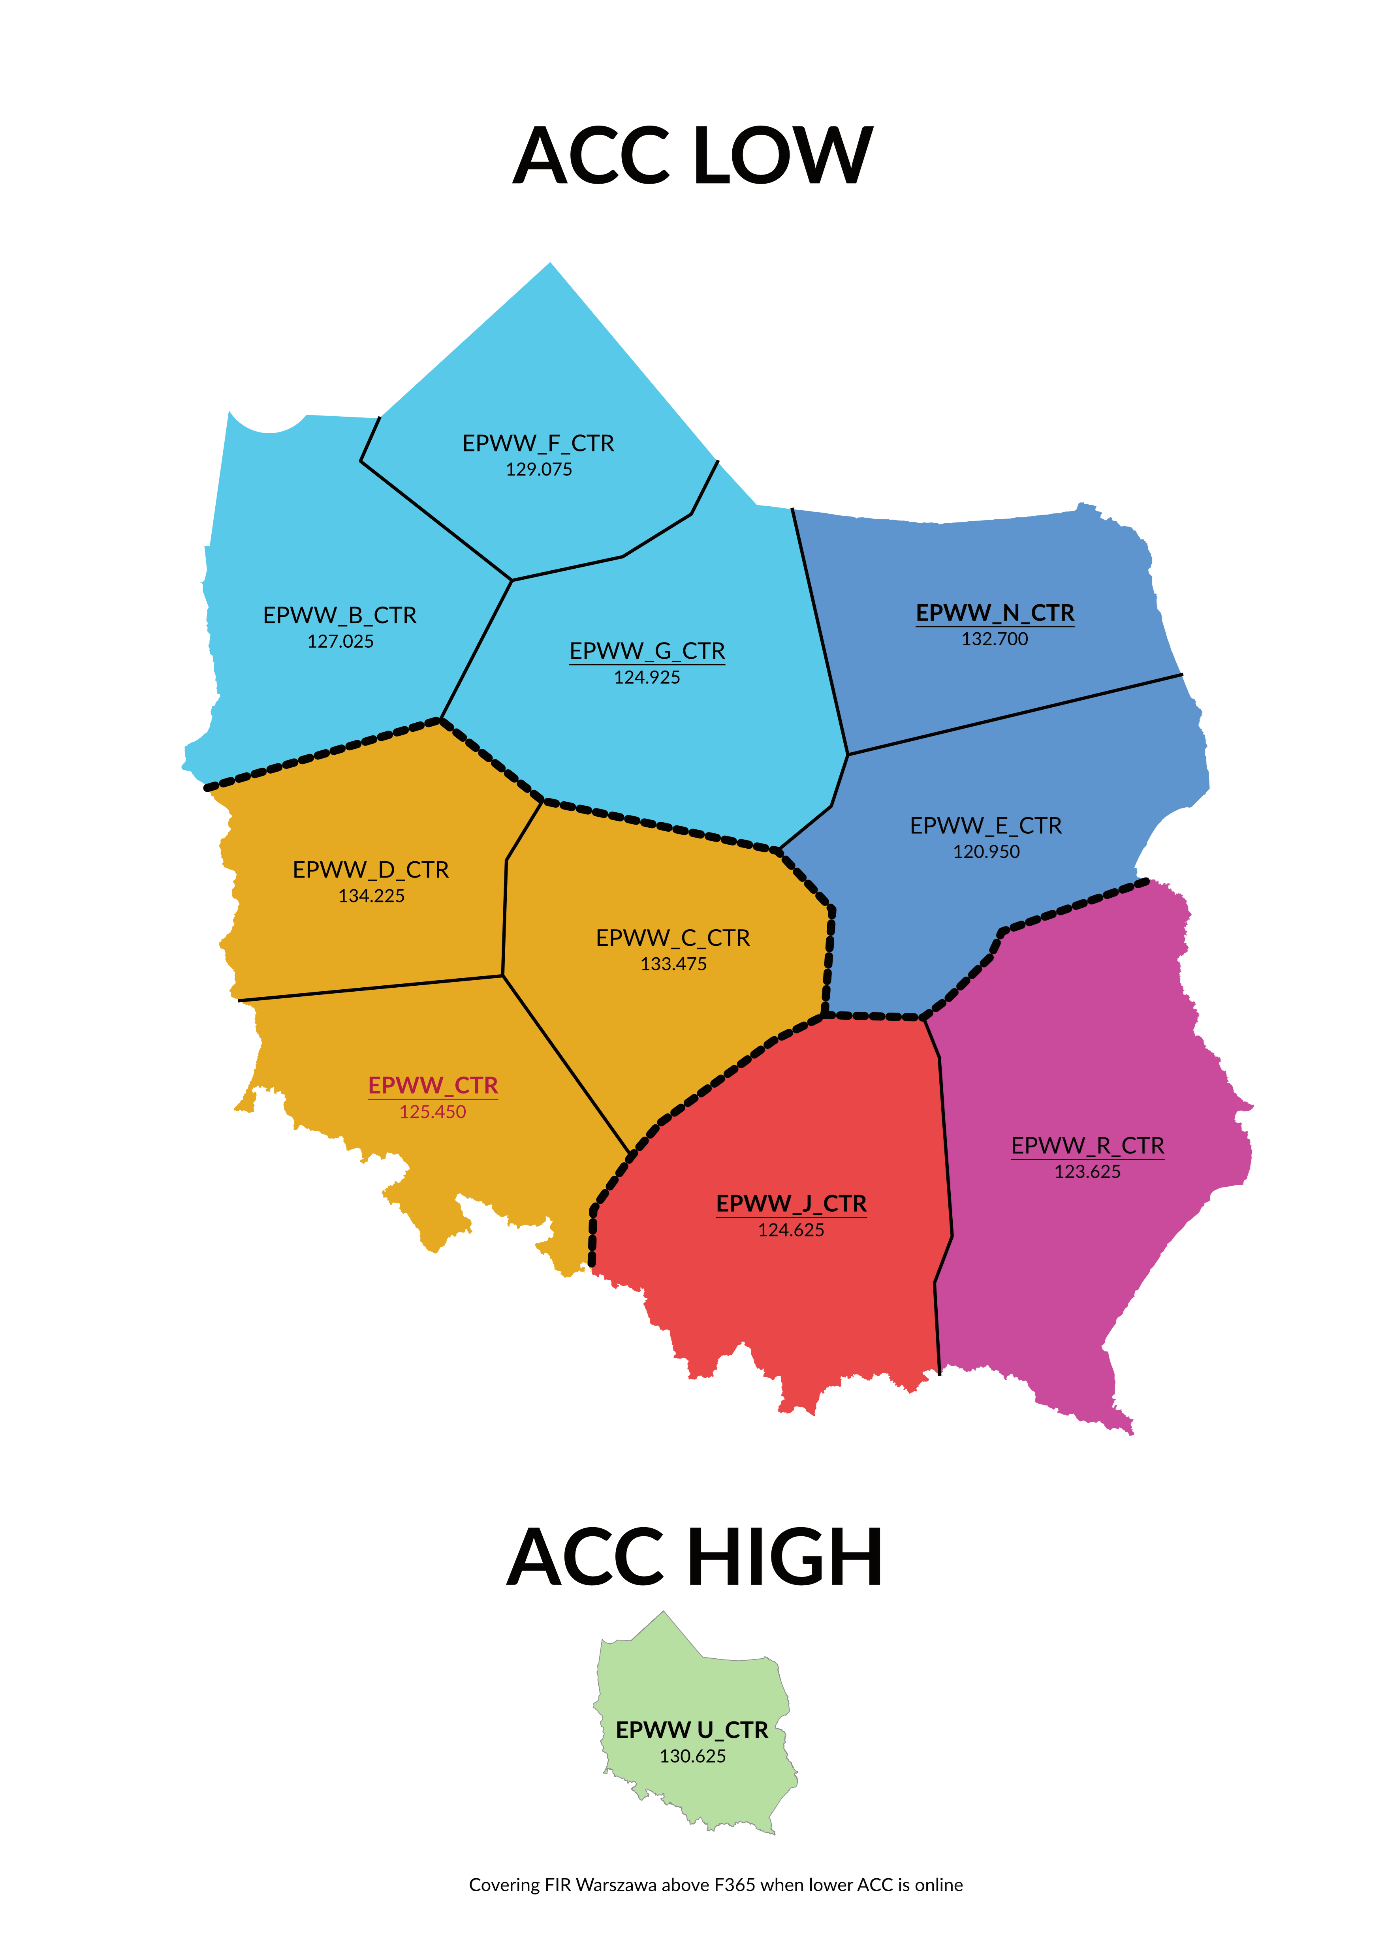
\includegraphics[width=0.8\textwidth]{acc_sectors.png}
  \caption{ACC sectors of vFIR Warszawa}
  \label{fig:acc:sectors}
\end{figure}

\section{Sector capacity}
\label{sec:acc:sectorcapacity}

\subsubsection{Single sectors}

\textbf{10} aircraft in the air at the same time, provided that no more than
\textbf{8} aircraft operate to a single airport.

\subsubsection{Sector blocks}

\textbf{15} aircraft in the air at the same time, provided that no more than
\textbf{12} aircraft operate to a single airport.

\subsubsection{Sector groups}

\textbf{20} aircraft in the air at the same time, provided that no more than
\textbf{12} aircraft operate to a single airport.

\subsubsection{Sector ALLFIR}

\textbf{20} aircraft in the air at the same time, provided that no more than
\textbf{8} aircraft operate to a single airport.

\section{Transfer of control between sectors}

Transfer of control between ACC sectors takes place as described in
\cref{sec:app:silentcoor}.

When ACC \textbf{\color{OliveGreen}UPPER\color{black}} is online, LOW sector controllers
issue initial climb instructions to FL~360. Transfer of control of an aircraft
cleared to climb to FL~360 to \textbf{\color{OliveGreen}UPPER\color{black}} controller
contains ATC release for further climb.

\textbf{\color{OliveGreen}UPPER\color{black}} controller issues initial descent
instructions to FL~370. Transfer of control of an aircraft cleared to descend to
FL~370 to appropriate lower controller contains ATC release for further descent.

\section{CPDLC}
\label{sec:acc:cpdlc}

ACC controllers may utilise CPDLC at their discretion. The recommended way of
using CPDLC is via the TopSky plugin.

CPDLC may be used in the Area Control Service for aircraft above
\textbf{FL~285}.

Designated LOGON codes for sectors are presented in \cref{tab:acc:cpdlc}.

\begin{table}[htbp]
  \centering
  \begin{tabular}{|c l|c|}
    \hline
    \multicolumn{2}{|c|}{\cellcolor{vred}\color{white}\textbf{Sector}}&\cellcolor{vred}\color{white}\textbf{LOGON}\\\hline
    \color{Orange}T ALLFIR & \tiny [EPWW\_CTR] & EPWW\\\hline
    \color{OliveGreen}UPPER & \tiny [EPWW\_U\_CTR] & EPWU\\\hline
    \color{ProcessBlue}B & \tiny [EPWW\_B\_CTR] & EPWB\\\hline
    \color{Orange}C & \tiny [EPWW\_C\_CTR] & EPWC\\\hline
    \color{Orange}D & \tiny [EPWW\_D\_CTR] & EPWD\\\hline
    \color{MidnightBlue}E & \tiny [EPWW\_E\_CTR] & EPWE\\\hline
    \color{ProcessBlue}F & \tiny [EPWW\_F\_CTR] & EPWF\\\hline
    \color{ProcessBlue}G & \tiny [EPWW\_G\_CTR] & EPWG\\\hline
    \color{vred}J & \tiny [EPWW\_J\_CTR] & EPWJ\\\hline
    \color{MidnightBlue}N & \tiny [EPWW\_N\_CTR] & EPWN\\\hline
    \color{vred}R & \tiny [EPWW\_R\_CTR] & EPWR\\\hline
  \end{tabular}
  \caption{CPDLC LOGON codes}
  \label{tab:acc:cpdlc}
\end{table}

Controllers providing CPDLC put the following information in their controller's
text ATIS: ``\textit{CPDLC \^{}F285 logon: [LOGON]}'', where \textit{[LOGON]} is
replaced by the LOGON code from \cref{tab:acc:cpdlc}.

%%% Local Variables:
%%% mode: latex
%%% TeX-master: "../main"
%%% End:
